% This version of CVPR template is provided by Ming-Ming Cheng.
% Please leave an issue if you found a bug:
% https://github.com/MCG-NKU/CVPR_Template.

%\documentclass[review]{cvpr}
\documentclass[final]{cvpr}

\usepackage{times}
\usepackage{epsfig}
\usepackage{graphicx}
\graphicspath{{Images/}}
\usepackage{amsmath}
\usepackage{amssymb}
\usepackage{listings}
% Include other packages here, before hyperref.

% If you comment hyperref and then uncomment it, you should delete
% egpaper.aux before re-running latex.  (Or just hit 'q' on the first latex
% run, let it finish, and you should be clear).
\usepackage[pagebackref=true,breaklinks=true,colorlinks,bookmarks=false]{hyperref}


\def\cvprPaperID{****} % *** Enter the CVPR Paper ID here
\def\confYear{CVPR 2021}
%\setcounter{page}{4321} % For final version only


\begin{document}

%%%%%%%%% TITLE
\title{Parallelizing Deep Neural Networks}

\author{Luis Guzman \\
University of Oregon\\
{\tt\small lguzmann@uoregon.edu}
\and
Steven Walton\\
University of Oregon\\

{\tt\small swalton2@cs.uoregon.edu}
% For a paper whose authors are all at the same institution,
% omit the following lines up until the closing ``}''.
% Additional authors and addresses can be added with ``\and'',
% just like the second author.
% To save space, use either the email address or home page, not both
}

\maketitle


%%%%%%%%% ABSTRACT
\begin{abstract}
\end{abstract}

%%%%%%%%% BODY TEXT
%\section{Introduction} % 

In the past decade, Artificial Neural Networks (ANNs) have become increasingly
popular, with advances in the area affecting almost every sector of computing.
Deep Neural Networks (DNNs) \--- deeper, more complex models than their
`shallow' counterparts \--- have progressed from being academic curiosities to
being the cornerstone of many modern technologies~\cite{deep_learning_overview},
with work showing that deeper networks tend to give better results than wide
networks~\cite{VGG}. Given this newfound relevance, many researchers have
devoted a lot of time optimizing these algorithms, constantly trying to improve
them for different accelerator technologies and platforms. Even long before
accelerators, many efforts in trying to parallelize neural networks were
made~\cite{10.1007/BFb0024235}.  While the new resurgence of machine learning
(ML) partially came from the generalized availability of hardware accelerators
like GPUs, there are still many innovations being made for CPUs. An example of
this is Facebook's new Speech-to-Text (stt) system that runs on
CPUs~\cite{fbcpu} and is aimed at home assistants that cannot rely on large and
power-hungry accelerators.  As ML algorithms are getting larger, there are also
continued efforts to apply machine learning techniques to simpler hardware.
Thus, for the foreseeable future, optimizing ML algorithms on various platforms
will remain an active area of research.

In this section we will discuss the various algorithms used in machine learning.
In Section~\ref{sec:ann} we will discuss Artificial Neural Networks and the
underlying theory behind them. In Section~\ref{sec:method} we will discuss how
we implemented our network and our design choices. In Section~\ref{sec:results}
we will discuss the results and the optimizations we achieved from our
parallelization efforts. Finally, in Section~\ref{sec:conclusions} we conclude
the work and summarize our findings.

\subsection{Artificial Neural Networks}\label{sec:ann}

This section presents the theory behind ANNs and the Gradient Descent (GD)
algorithm that is commonly used to train them.

\subsubsection{Perceptrons}

The Perceptron, also referred to as ``neuron'', is the basic unit of an ANN. It
is a mathematical function that was inspired by the biological neurons in the
human brain~\cite{rosenblatt1958perceptron}. Its mathematical formula is presented in Equation~\ref{eq:perceptron}. It consists of a dot product between a feature vector $x$
and a weights vector $w$. The resulting dot product of these vectors is then fed
into a function $g$ known as \textit{activation}~\cite{activation_functions} which yields the output
$\hat{y}$ of the neuron.

\begin{align}
    \hat{y} = g\left(\sum^n_{i=0} w_ix_i\right)
    \label{eq:perceptron}
\end{align}

Perceptrons can be used to solve regression (estimating real values) or
classification problems (discrete number of classes). The feature vectors are
obtained directly from the function being estimated or the dataset being
classified. The weights vector can be initialized to a vector of zeros, however,
it is common to initialize it using random numbers in the range $[0,1)$ drawn
from a uniform distribution. By providing random initializations networks
typically converge faster and generalize better.

As for the activation function, Figure~\ref{fig:activations} presents a few
examples of commonly used ones~\cite{activation_functions}. The bottom-right image in
Figure~\ref{fig:activations} shows an example of a linear activation in the form
of the Identity function. The other three examples represent non-linear
activations: the Sigmoid (bottom-left) function yields an output between 0 and
1; the Hyperbolic Tangent function (up-left) has an output between -1 and 1; and
the Rectified Linear Unit, or ReLU, (up-right) is a modified Identity that
changes negative values to 0.

\begin{figure}[!htbp]
    \centering
    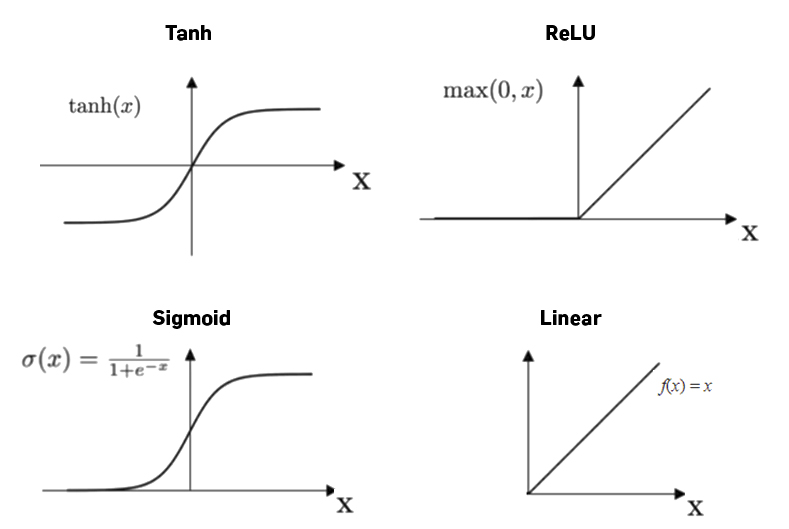
\includegraphics[width=.5\textwidth]{Images/activations.jpg}
    \caption{Examples of activation functions.}
    \label{fig:activations}
\end{figure}

The activation function plays a crucial role because it actually determines the
sort of problems that a perceptron is able to solve. If a linear (Identity,
Step, Sign) activation function is used, a single perceptron is only able to
solve ``linearly separable'' problems, that is, problems in which the classes
can be successfully separated by a hyper-plane (Figure
\ref{fig:linear_vs_non_linear} left). On the other hand, by using a non-linear
(Sigmoid, Tanh, ReLU) activation a more flexible decision boundary is created
and, thus, more complex problems can be solved (Figure
\ref{fig:linear_vs_non_linear} right).

\begin{figure}[!htbp]
    \centering
    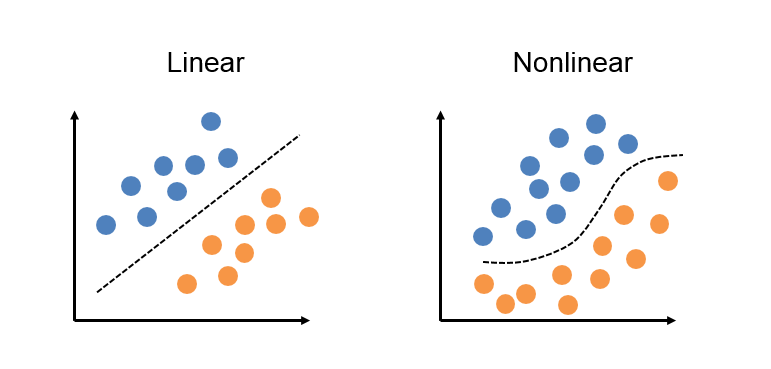
\includegraphics[width=.5\textwidth]{Images/linear_vs_non_linear.png}
    \caption{Linearly-separable vs non-linearly separable.}
    \label{fig:linear_vs_non_linear}
\end{figure}

\subsubsection{Training Perceptrons with Gradient Descent}
 
It is safe to assume that the initial output of the perceptron $\hat{y}$,
obtained with the initial state of the weights vector, will be different than
the expected output $y$ (label). So, in order to improve these predictions, the
perceptron needs to be ``trained''. Training a perceptron basically means
iteratively modifying the weights vector so that the outputs start to
approximate the expected ones. This training process is illustrated in
Figure~\ref{fig:perceptron_train}: using the the expected output $y$ and the
obtained output $\hat{y}$ an error measure is computed and used to modify the
weights. This process is repeated until the outputs fulfill a  given convergence
criteria or a maximum number of iterations is reached.
 
\begin{figure}[!htbp]
    \centering
    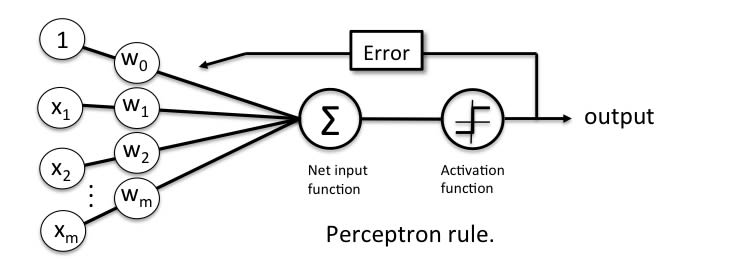
\includegraphics[width=.5\textwidth]{Images/perceptron_learning.jpg}
    \caption{Perceptron training.}
    \label{fig:perceptron_train}
\end{figure}

The Gradient Descent (GD) algorithm~\cite{gradient_descent} is an optimization technique that is used to
train perceptrons. The main idea behind GD is to update the weights in the
direction of the gradient of the function used to compute the error between the
perceptron's outputs and the expected ones. This function is commonly referred
to as \textit{Loss} function~\cite{loss_functions}. The actual problem being solved determines the
type of loss function that should be used. For example, in regression problems
the Mean Squared Error (MSE) loss function is a typical choice. For binary
classification problems, Binary Cross-Entropy loss or Hinge loss are good
options. In multi-class classification problems, Cross-Entropy loss is the
default alternative.

The general formula for the GD method is shown in Equation~\ref{eq:gd_formula}. First, the derivative of the chosen loss function $L$ with respect to the weights vector $w$ is obtained. Then it is multiplied by a scalar parameter $\gamma$ known as \textit{learning rate}. Finally, the weights are updated using this product.

\begin{align}
    w = w - \gamma \frac{d}{d_w}L
    \label{eq:gd_formula}
\end{align}

While the formula for GD is straightforward, obtaining the derivative of the
loss function with respect to the weights is not always trivial as the chain
rule of derivatives is needed. For example, Equation~\ref{eq:bce_loss} shows the
mathematical formula of the Binary Cross-Entropy loss function.

\begin{align}
    L(w) = y * \log(\hat{y}) + (1 - y) * \log(1 - \hat{y})
    \label{eq:bce_loss}
\end{align}

If we assume a perceptron using the sigmoid activation function, the derivative
of the loss is obtained in the following manner:

\begin{align}
    d &= w^T x \\
    \hat{y} &= \sigma(d) = \frac{1}{1 + e^{-d}} \\
    \frac{\partial L(w)}{\partial w} &= \frac{\partial L(w)}{\partial \hat{y}} \cdot \frac{\partial \hat{y}}{\partial d} \cdot \frac{\partial d}{\partial w}\\
    \frac{\partial L(w)}{\partial \hat{y}} &= -\left(\frac{y}{\hat{y}} - \frac{1
    - y}{1 - \hat{y}}\right) = \frac{\hat{y} - y}{\hat{y}(1-\hat{y})} \\
    \frac{\partial \hat{y}}{\partial d} &= \hat{y}(1 - \hat{y}) \\
    \frac{\partial d}{\partial w} &= x \\
    \frac{\partial L(w)}{\partial w} &= x^T(\hat{y}-y)
\end{align}

There are some variations to the GD algorithm, each with its own strengths and
weaknesses. In Stochastic Gradient Descent (SGD)~\cite{gradient_descent}, the weights are updated for
each training sample in the dataset, i.e. the output of one feature vector is
obtained, the derivative of the loss function for that output is computed, and
the weights are updated according to the GD formula. This version is, of course,
suitable for online training or when the training dataset is so big that it
cannot fit in memory all at once. However, the constant weight updates produce a
the chaotic behaviour shown in Figure~\ref{fig:sgd} as each training sample
attempts to pull in its own direction.

\begin{figure}[!htbp]
    \centering
    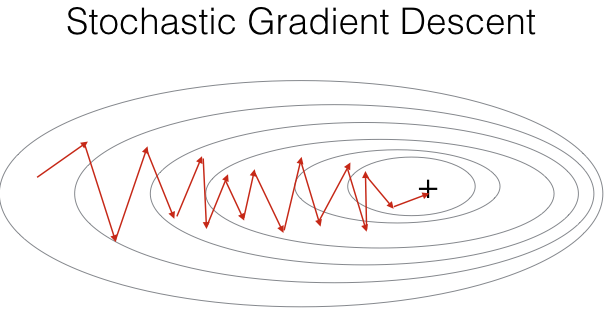
\includegraphics[width=.4\textwidth]{sgd.png}
    \caption{SGD convergence behaviour.}
    \label{fig:sgd}
\end{figure}

The (Mini) Batch Gradient Descent (BGD)~\cite{gradient_descent} variation instead splits the training
samples into small-sized batches and only updates the weights once per each
batch. Thus, using BGD makes the algorithm behave more smoothly with less
pronounced changes in its path towards convergence as it is shown in
Figure~\ref{fig:bgd}.

\begin{figure}[!htbp]
    \centering
    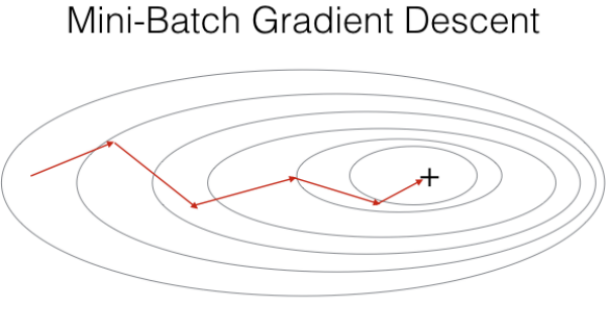
\includegraphics[width=.4\textwidth]{bgd.png}
    \caption{BGD convergence behaviour.}
    \label{fig:bgd}
\end{figure}

\subsubsection{Multi-layer Perceptrons}

There are, of course, limitations to what a single perceptron can accomplish no
matter the activation function used. Figure~\ref{fig:unsolvable} presents one of
such cases in which a classification problem cannot be solved by a single
perceptron, which is because multilayer perceptron networks are universial
approximators~\cite{HORNIK1989359}. The dataset shown
in the figure contains points in two dimensions labeled as two distinct classes
identified by the colors blue and orange. As can be observed, the blue class is
``contained'' within the orange class and, as such, it is impossible for a
single perceptron to define a decision boundary, even a non-linear one, that
will correctly classify all of the points. 

\begin{figure}[!htbp]
    \centering
    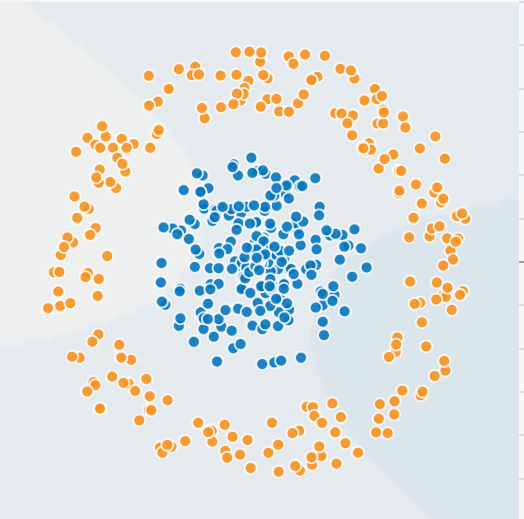
\includegraphics[width=.35\textwidth]{Images/circles.png}
    \caption{Class contained within the other.}
    \label{fig:unsolvable}
\end{figure}

Figure~\ref{fig:one_perceptron} presents the decision boundary created by a
single perceptron using a sigmoid activation. In the figure, it can be observed
that the resulting decision boundary correctly classifies most of the blue-class
points. However, it incorrectly classifies the vast majority of the orange-class
points.

\begin{figure}[!htbp]
    \centering
    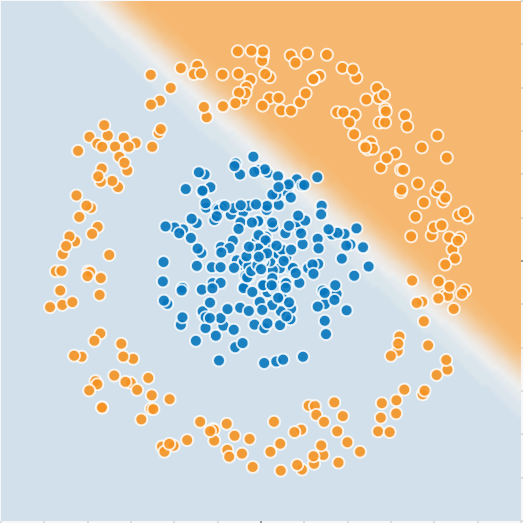
\includegraphics[width=.35\textwidth]{Images/circles_perceptron.png}
    \caption{One perceptron solution.}
    \label{fig:one_perceptron}
\end{figure}

In problems such as the this one using an ANN, also known as Multi-Layer
Perceptrons (MLPs), becomes necessary. A MLP consists in several perceptrons
connected together to form a ``network''. In the literature, there exist
multiple ways in which the perceptrons can be arranged to form different
architectures~\cite{deep_learning_overview}. However, in this work we focus on
the architecture known as ``Feed-Forward Neural Network'' (FFNN)~\cite{ffnn},
shown in Figure~\ref{fig:ffnn}. In FFNNs, all neurons in one layer are connected
to all of the neurons in the following layer, hence the name Feed-Forward.

\begin{figure}[!htbp]
    \centering
    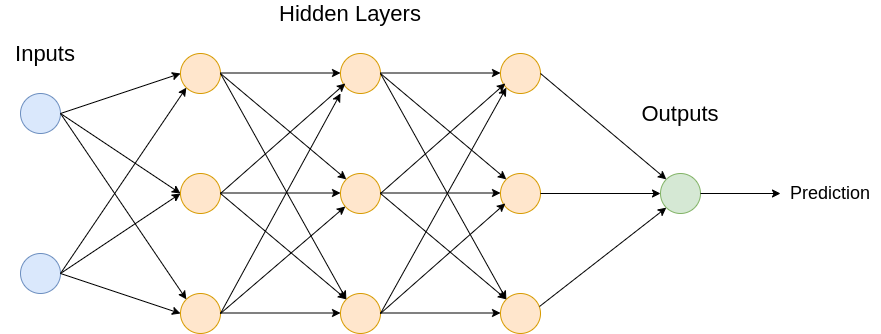
\includegraphics[width=.5\textwidth]{Images/mlp.png}
    \caption{Structure of a Feed-Forward Neural Network.}
    \label{fig:ffnn}
\end{figure}

In a FFNN, perceptrons are organized into 3 types of layers: input, hidden, and
output layers.  Input layers receive the feature vectors as inputs and connect
to the first hidden layer. Hidden layers are intermediate layers that make up
for the bulk of the network. Finally, the output layer is tasked with producing
the result of the network. 

Each layer in a FFNN can have a different number of neurons, and each neuron
within a layer can have a different activation function. It is usual, however,
for neurons in the same layer to have the same activation. 

The number of neurons in the output layer and their activation types depend on
the type of problem being solved. For a regression problem, the network only has
one output neuron, usually with an identity linear activation. In binary
classification problems, one output neuron is sufficient. A sigmoid activation
is also usually used in these cases~\cite{Cybenko1989ApproximationBS}, with
labels 0 and 1 used to represent the two classes. For multi-class
classification, the number of neurons in the output layer matches the number of
classes being identified and a \textit{Softmax}~\cite{pattern_recognition}
(Equation \ref{eq:softmax}) operation is applied to the results of the output
layer neurons' to create a probability distribution vector. The class prediction
is then obtained by obtaining the argmax of such probability vector.

\begin{align}
    \textit{Softmax}(\hat{y}_i) = \frac{e^{\hat{y}_i}}{\sum\limits_j e^{\hat{y}_j}}
    \label{eq:softmax}
\end{align}

Figure~\ref{fig:mlp_solved} shows the decision boundary created by a FFNN with 2
hidden layers of 3 neurons each trained on the dataset discussed previously.

\begin{figure}[!htbp]
    \centering
    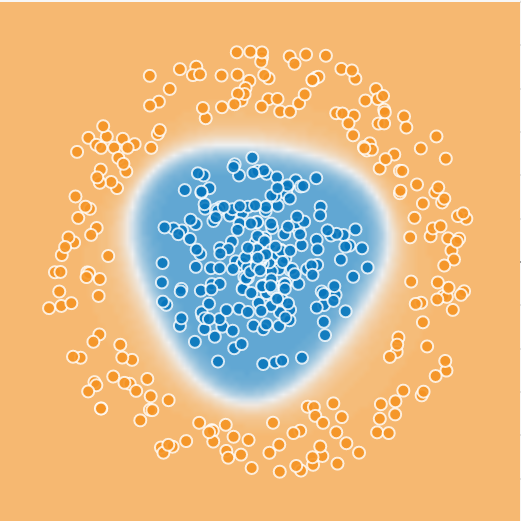
\includegraphics[width=.35\textwidth]{Images/circles_solved.png}
    \caption{Solution with MLP.}
    \label{fig:mlp_solved}
\end{figure}

To make predictions in a FFNN network, the outputs of each layer, also referred
to as \textit{activations}, are obtained sequentially. The activations of the
input layer, obtained using the feature vectors, are in turn used as the inputs
for the first hidden layer. This process known as the \textit{Forward Pass} is
repeated until the activation of the output layer is computed
(Figure~\ref{fig:forward}).

\begin{figure}[!htbp]
    \centering
    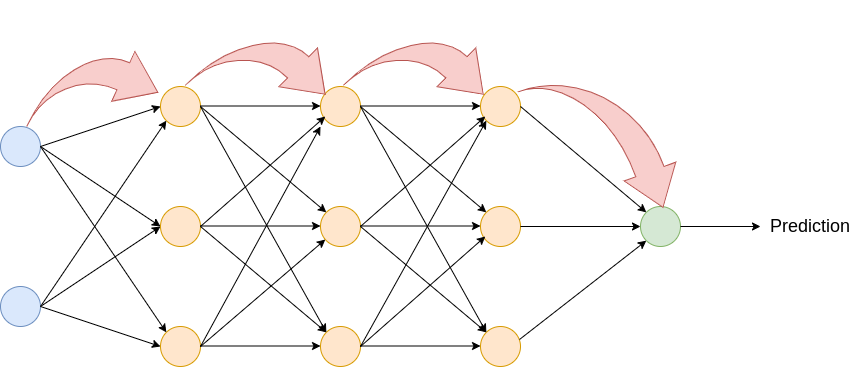
\includegraphics[width=.5\textwidth]{Images/forward_pass.png}
    \caption{Forward pass.}
    \label{fig:forward}
\end{figure}

When using BGD, the forward pass through a FFNN becomes a series of matrix
multiplications. The inputs become a matrix with dimensions $[\textit{Batch\_Size} \times
\textit{\#\_Features}]$ and at each layer, the activations are obtained by multiplying
the input matrix by the weight matrix.
Equations~\ref{eq:forward1}-\ref{eq:forward4} show the forward pass for a
network with 3 hidden layers and one output layer. Note: these equations
purposely omit the neuron's activations as the objective is to highlight the
matrix operations.

\begin{align}
    h_{1_{act}} &= \textit{Inputs} \cdot W_{h_1} \label{eq:forward1}\\
    h_{2_{\textit{act}}} &= h_{1_{\textit{act}}} \cdot W_{h_2} \label{eq:forward2}\\
    h_{3_{\textit{act}}} &= h_{2_{\textit{act}}} \cdot W_{h_3} \label{eq:forward3}\\
    \hat{y} &= h_{3_{\textit{act}}} \cdot W_{O}
    \label{eq:forward4}
\end{align}

Updating the weights in a FFNN is more complex than with a single perceptron.
The loss function merely determines the error at the output layer of the
network. It is then necessary to propagate such error through every layer in the
network all the way back to the input layer. To achieve this, the
\textit{Backpropagation} algorithm~\cite{backprop} is used (Figure~\ref{fig:backprop}).

\begin{figure}[!htbp]
    \centering
    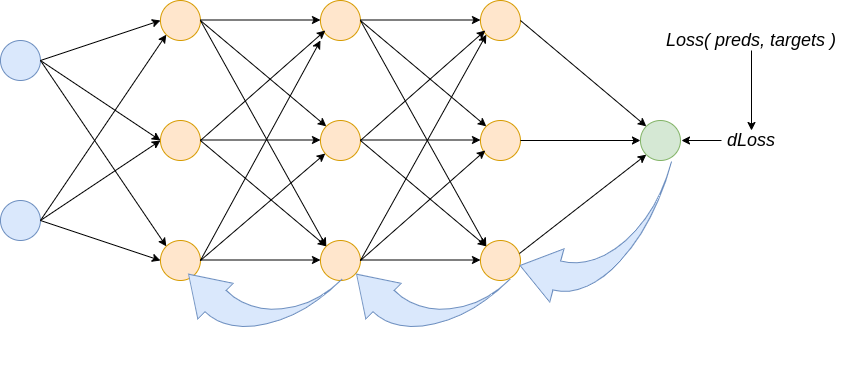
\includegraphics[width=.5\textwidth]{Images/backprop.png}
    \caption{Backpropagation of the error.}
    \label{fig:backprop}
\end{figure}

Once the derivative of the loss function is obtained at the output layer, the
error is propagated back to the preceding layer by multiplying it by the output
layer weights. This same procedure is repeated until the error has reached the
input layer (Equations~\ref{eq:backprop1}-\ref{eq:backprop4}). Note: as before,
these equations omit the derivative of the activation functions as the focus
should be on the matrix operations. 

\begin{align}
    O_{\textit{error}} &= dL_\textit{oss} \label{eq:backprop1}\\
        h_{3_{\textit{error}}} &= O_{\textit{error}} \cdot (W_{O})^T \label{eq:backprop2}\\
        h_{2_{\textit{error}}} &= h_{3_{\textit{error}}} \cdot (W_{h_3})^T \label{eq:backprop3}\\
        h_{1_{\textit{error}}} &= h_{2_{\textit{error}}} \cdot (W_{h_2})^T \label{eq:backprop4}
\end{align}

After the errors for all layers have been computed, the weights can be updated
using the GD formula (Equations~\ref{eq:update1}-\ref{eq:update4}).

\begin{align}
    W_{h_1} &= W_{h_1} - \gamma ((I_\textit{nputs})^T \cdot h_{1_{\textit{error}}}) \label{eq:update1} \\
    W_{h_2} &= W_{h_2} - \gamma ((h_{1_{\textit{act}}})^T \cdot h_{2_{\textit{error}}}) \label{eq:update2} \\
    W_{h_3} &= W_{h_3} - \gamma ((h_{2_{\textit{act}}})^T \cdot h_{3_{\textit{error}}}) \label{eq:update3} \\
    W_{O} &= W_{O} - \gamma ((h_{3_{\textit{act}}})^T \cdot O_{\textit{error}}) \label{eq:update4}
\end{align}



\section{Methodology}\label{sec:method}

For this project we set out to design a robust framework to build neural
networks, drawing inspiration form industry and academic standards like PyTorch
and TensorFlow. With this idea in place we set out to make a framework that
allowed for 1) arbitrary network sizes 2) easy integration of different network
features, such as different forms of gradient descent or regularizers, and 3)
modularity that would allow for further expandability. We found these features
to be important for several reasons, besides trying to mimic something that
would be useful and not a one-trick pony. By having arbitrary network sizes this
would allow us to test on a wide variety of datasets. Furthermore we had
suspicions when starting the project that a network that could be trained well
on simple datasets may also not be large enough to benefit much from
parallelization. By allowing for arbitrary network sizes this would allow us to
better test as the project progressed. Easy integration of new features and
extendability this allowed us to quickly test more ideas and expand the project,
as we did not know how much we would be able to implement. With this unknown
factor and a short deadline being able to quickly add new features without major
code rewrites is a valuable tool. 

To create these features we broke out the network into multiple classes, again
drawing on inspiration from PyTorch and HPC tools like VTK-m. We separated out
all our math functions into one class, individual linear layers into another
class, and finally the model into a super class. With this construction we could
implement networks of arbitrary sizes, extend them, modify our algorithms, and
so on with little conflict. In Figure~\ref{fig:model} we show the code required
to generate a simple model that will accurately classify the Moons Dataset. As
can be seen, this allows for a very similar construction style to that of
PyTorch, where one simply needs to define the Linear Layers with the input and
output size and how they are connected. Similarly our Sequential class
determines how to connect all the nodes together and creates all the connections
that will be needed for the Forward and Backwards functions. In our example the
construction under the ``creating layers'' section is similar to PyTorch's model
constructor and our ``Adding layers to the model'' section is similar to
PyTorch's ``forward'' function.

\begin{figure}[ht]
\begin{lstlisting}[language=C++,
                   directivestyle={\color{black}},
                   emph={size_t, LinearLayer, defineModel, Sequential, float},
                   emphstyle={\color{blue}}]
void defineModel(Sequential &model, 
                 float learning_rate)
{
    //creating layers
    LinearLayer i_layer(2,3, 
                   learning_rate, 
                   model.getBatchSize());
    LinearLayer h1(3,3, 
                   learning_rate, 
                   model.getBatchSize());
    LinearLayer h2(3,3, 
                   learning_rate, 
                   model.getBatchSize());
    LinearLayer o_layer(3,1, 
                   learning_rate, 
                   model.getBatchSize());

    //Adding layers to the model
    model.add(i_layer);
    model.add(h1);
    model.add(h2);
    model.add(o_layer);
}
\end{lstlisting}
\caption{Example model construction}
\label{fig:model}
\end{figure}

In a similar fashion we designed the rest of the network. This was particularly
helpful in that the math library was similarly fashioned. By the arbitrary input
sizes we could simply focus on the operations that took the most time.
Similarly, this made it simpler to optimize because we could directly find which
mathematical operations were performing the most work and that it matched our
intuition. 

While this all worked as expected for our OpenMP implementation this methodology
gave us problems when we started to build our CUDA implementation. With our
inexperience in CUDA we had assumed that porting the majority of the network
would be similar and we would only need to create new kernels for our math
functions. By the time we had started to really understand CUDA we had a fully
developed and working OpenMP implementation that was working well and showed
significant performance increases through parallelization. We learned a valuable
lesson about how good design choices for a CPU implementation did not
necessarily equate to good design choices for GPU acceleration. Had we had more
CUDA experience, or any, going into the project we would have likely made
different design choices. Had we more time to spend on this project we would
have spent more time learning about how to implement structures in CUDA and that
would have helped integrate the designs. 

\subsection{Computing Resources}
We performed our experiments on one system, UO's Alaska in the CDUX group. All
OpenMP operations were performed on the head node, which has 2 Intel Xeon
E5-2667v3's that have 8 physical cores and 16 threads, each, for a total of 32
threads. All CUDA operations were performed on compute node 2 which has a single
Intel Xeon E5-1650 with 6 physical cores and 12 threads as well as an Nvidia
GeForce RTX 2080Ti. 

\section{Results}\label{sec:results}
In this section we investigate the how parallelisms affected our program. We
break the report into three sections. In the first section (Sec~\ref{sec:r-opt})
we discuss the optimization techniques we performed, in the second
section (Sec~\ref{sec:r-omp}) we discuss our OpenMP implementation, and finally
in the third section (Sec~\ref{sec:r-cuda}) we discuss our CUDA implementation. 

\subsection{Optimizaton}\label{sec:r-opt}
In common fashion, before we start implementing parallelization we first started
optimizing the serial implementation of our code. We do this first because many
optimization techniques are about memory access and reducing the number of times
an address is accessed. This helps with both OMP and CUDA parallelization
because in both cases we will still want to reduce our memory footprint. While
CUDA optimization won't see as much benefits from this exercise, as CUDA
optimization is more dependent upon multi-dimensional memory access, using
blocks and grids, it will still be beneficial overall. 

To do this first took our working code and profiled it. Because our code allows
for arbitrary sized neural networks we increased the number of hidden layers and
neurons to get better profiling, though this decreased our accuracy. 
%We
%increased to 5 hidden layers (7 total) and each hidden layer had 300 neurons.
%This was a fair balance between taking too long to compute and not having enough
%work to perform. 
Profiling the code this way we looked for areas where we could
first pre-allocate memory, This had significant effects in the speedup. We then
looked for loops where we could reduce redundant computation, for example
calculating the vector size every loop iteration. An example of this shown in 
Figure~\ref{fig:opt}. These types of optimizations significantly improved our
results. 

\begin{figure}[ht]
(a)
\begin{lstlisting}[language=C++,
                   directivestyle={\color{black}},
                   emph={size_t},
                   emphstyle={\color{blue}}]
for(size_t i = 0; i < vec.size(); ++i)
   for(size_t j = 0; j < vec[0].size(); ++j)
      computation
\end{lstlisting}
(b)
\begin{lstlisting}[language=C++,
                   directivestyle={\color{black}},
                   emph={size_t},
                   emphstyle={\color{blue}}]
size_t v_size = vec.size();
size_t v0_size = vec[0].size();
for(size_t i = 0; i < v_size; ++i)
   for(size_t j = 0; j < v0_size; ++j)
      computation
\end{lstlisting}
\caption{Reducing loop lookups. (a) unoptimized (b) optimized}
\label{fig:opt}
\end{figure}

Previous to these, and other, optimizations our functions were not near the
worst performers according to $gprof$. After these we had our matrix multiply
function, our transpose, and our vector addition near the top. All these
optimizations ensured that there was proper pipelining and that we could fully
exploit our parallelism. One final optimization that we did is optimize the
matrix multiplication to get the best indexing we could, over a naive version
that was initially implemented. This provided the largest speedup.

\subsection{OpenMP}\label{sec:r-omp}
After we have ensured that proper pipelining and serial optimization are
implemented the next task is to parallelize. Because of the shared memory in OMP
our optimizations in Section~\ref{sec:r-opt} we only have to access these memory
points once and then we can share that memory across the threads. Because most
of our computation was in the form of vector or matrix operations we can
pipeline like above, share the memory, and parallelize the outer most loop so
that we can exploit the faster stride on the inside of the loop, since those
points are contiguous in memory and the outer loop isn't. 

To parallelize our code we focused on our math library, which held all our
mathematical functions and performs all our tensor operations. We investigated
parallelizing every operation and found that most operations had little to no
effect. A major hurdle we had was that we found that we needed hundreds of
neurons and a fair amount of layers for parallelism to create several hidden
layers. For the problems we are solving, such as the half moon, this is far too
large to learn the dataset and will over fit. For example, to learn the half
moon dataset we only needed 2 input neurons, a single hidden layer with 3 neurons,
and an output layer. With this network, not even a ``deep'' neural network,
we quickly converged on the answer, typically below 100 epochs. The
parallelization helps significantly more when increasing the number of neurons
as opposed to the depth of the network, or the number of hidden layers. But
since our goal was to build a framework, similar to PyTorch, we just needed to
test the parallelization rather than solve a specific problem. Thus we created
experiments with 300 neurons in each hidden layer and 5 hidden layers. We found
this to be a good balance between the program not taking too long to run and
having enough work to see speedups from parallelism. 

To see the effect of parallelism we perform a small ablation study to see what
was needed for speedup and what wasn't. We show the results of this in
Figure~\ref{fig:omp}. As we can see here, the matrix multiply parallelization
had the largest impact on speedup. Without this the other cases actually
increase as the number of CPUs increase. Note that we are parallelizing most
functions and these do have some overhead. Interestingly we find that the run
without either matrix multiply nor vector add implemented runs slightly faster
than when just matrix multiply is removed. We believe that this is because of
the lack of work. One other factor to note is that at 16 threads we note a
slight increase, where previously we were strictly decreasing. This is because
our machine has 2 Xeons with 8 physical cores (a total of 16) but they have 2
threads per core. Some work performs better on physical cores rather than
hyper-threading, which is why it is turned off in many HPC applications, and we
see that this holds true here. 

\begin{figure}[ht]
\centering
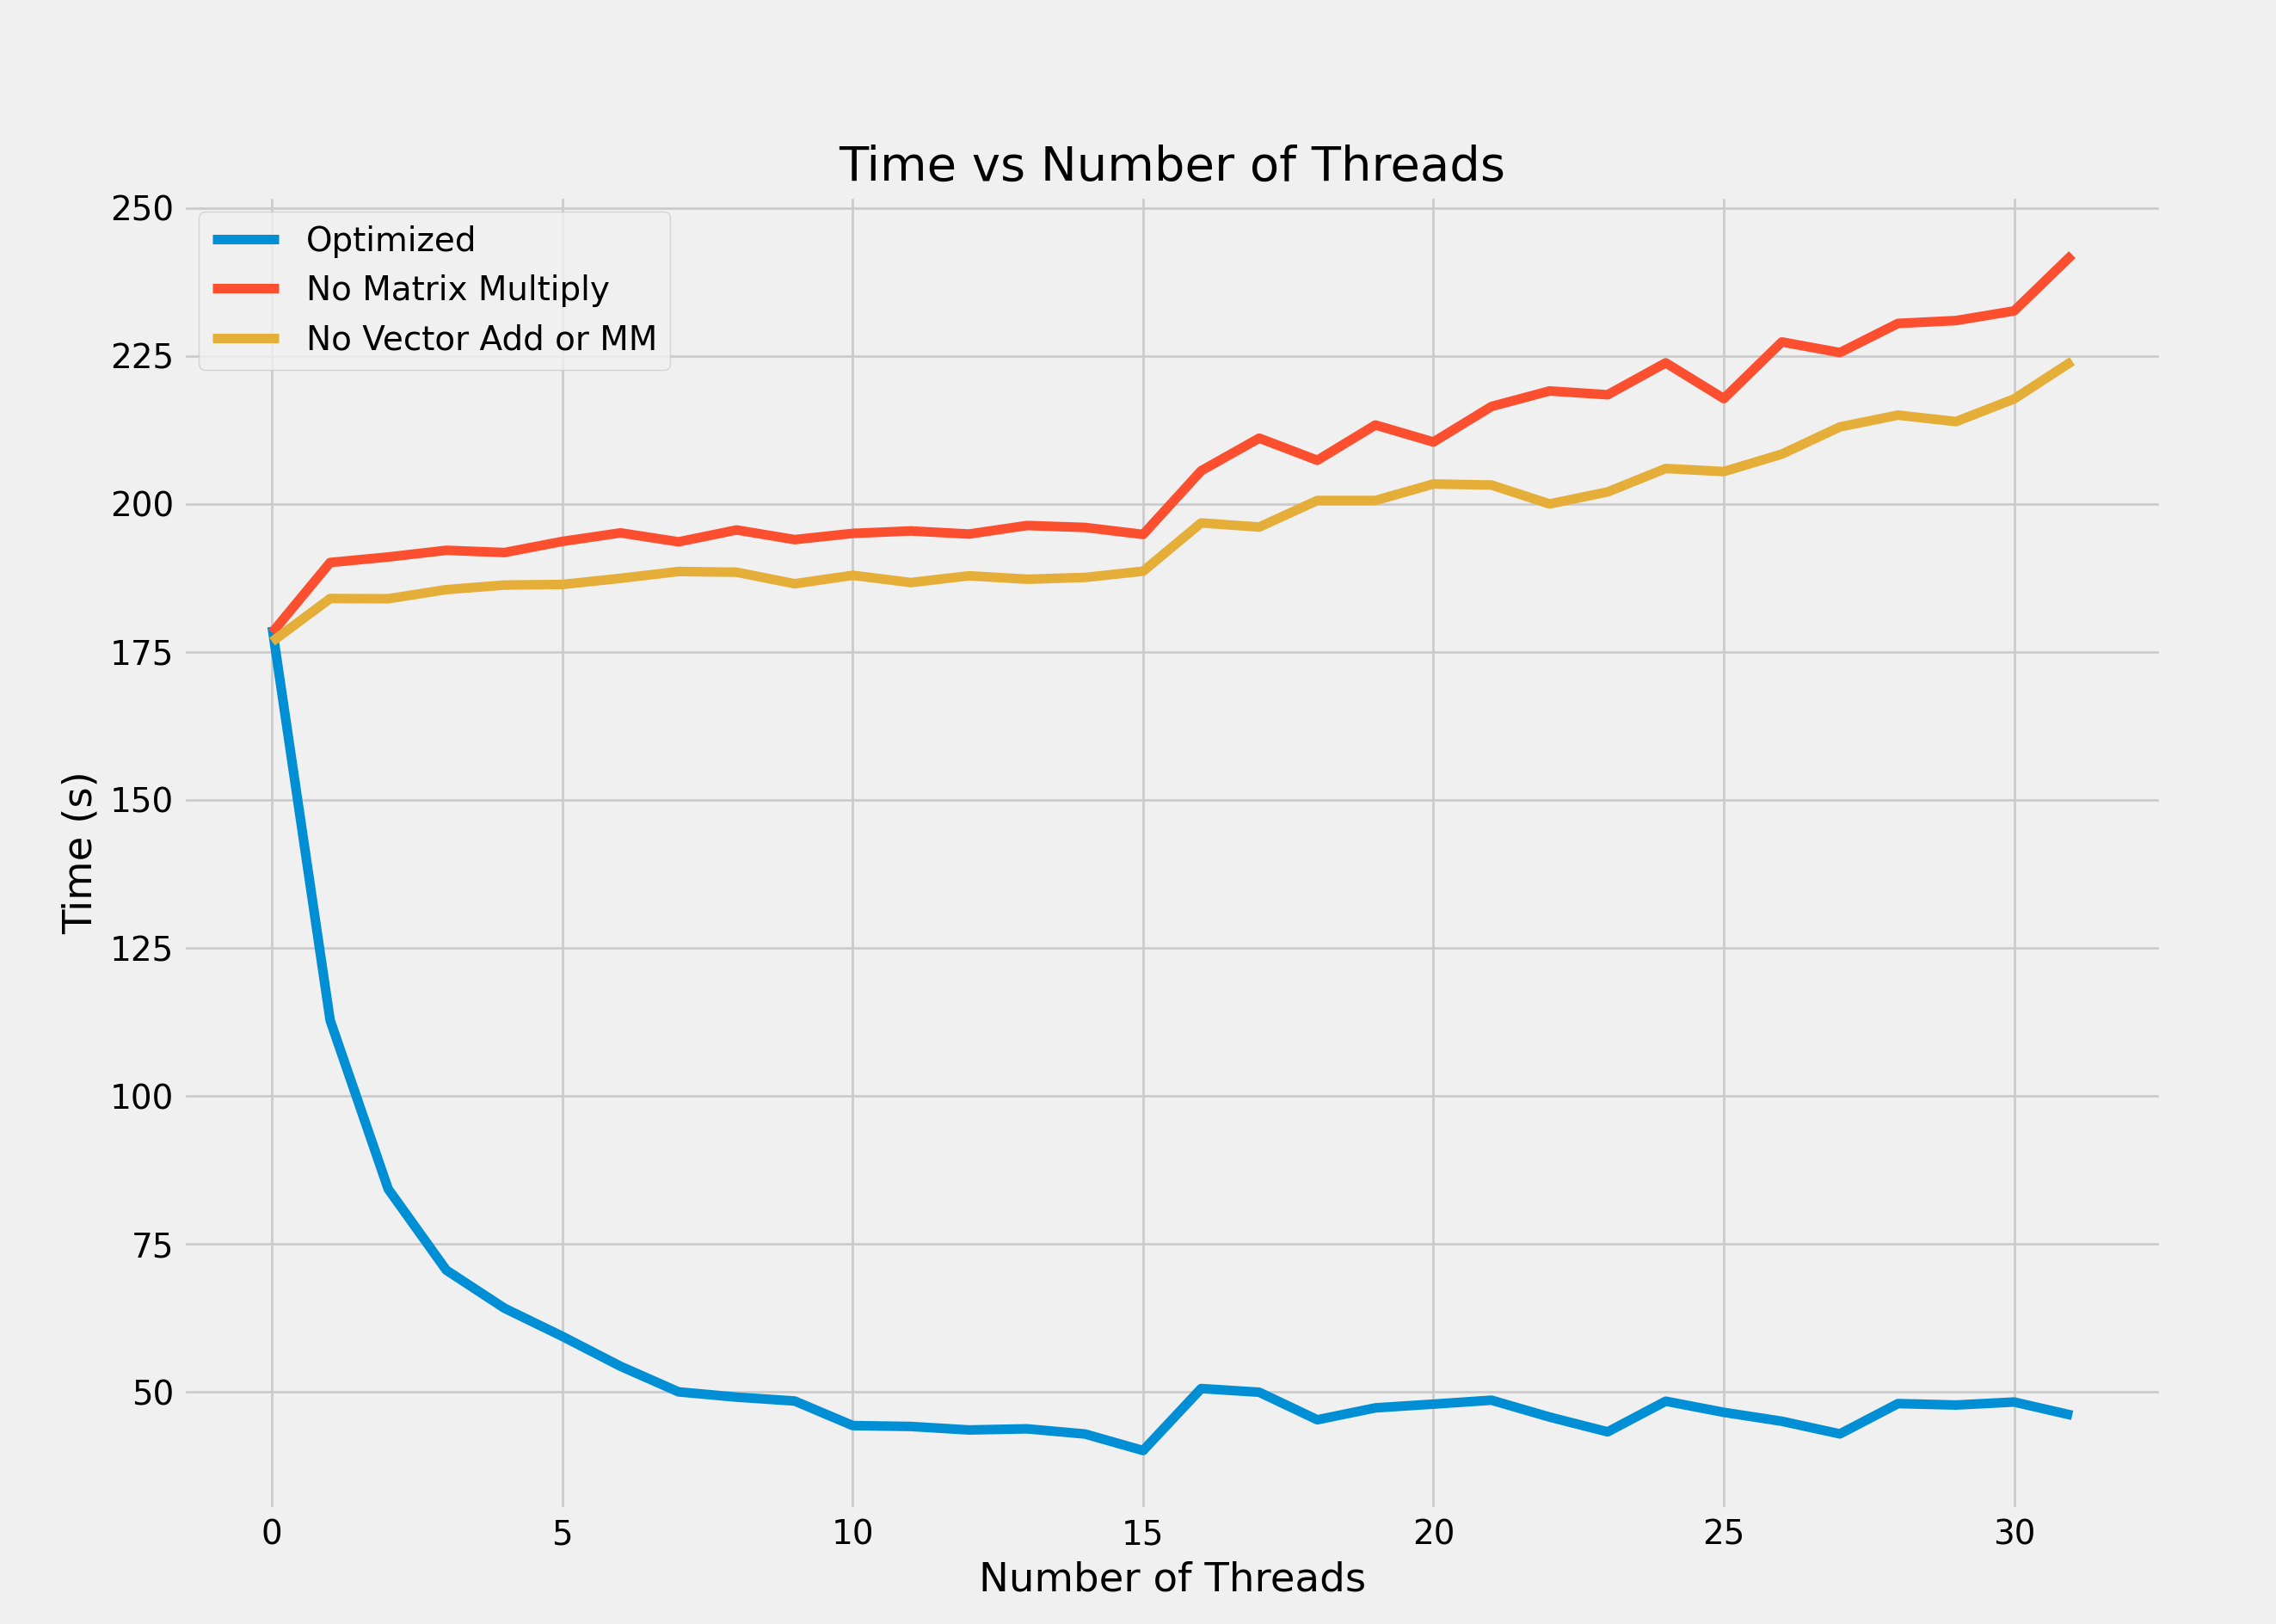
\includegraphics[width=\linewidth]{omp.png}
\caption{Comparison of how different functions affect parallelization results,
    using OpenMP}
    \label{fig:omp}
\end{figure}

Additionally we look at our matrix multiplication vs using a cache optimized
version. We can see the results in Figure~\ref{fig:cache}. We see here that we
don't get speedup even though we are better cache aligned. The reason, again,
for this is because the lack of work as well as the size of the matrices. The
problem with this is that our matrices aren't very large. Which we have many
rows, we don't have very many columns. This causes no real speedup from blocking
the matrices up because at most we can block is 2. This ends up causing more
cache misses than hits. We predict that even MNIST wouldn't give us a
significant improvement. We do not expect this to provide significant speedups
until we start working on larger problems like ImageNet. Additionally we had
problems with the block matrices because our matrices were inconsistent sizes,
including sometimes vectors. Vectors happened when at the final layer. This made
for very inconsistent results. We got the best results when blocking by 2 and
checking if our matrix sizes were even first. 

\subsection{CUDA}\label{sec:r-cuda}
We were unfortunately unable to get the entire model into CUDA but we still
wanted to provide some motivation as to how GPU acceleration would help with our
problem. Knowing that PyTorch and TensorFlow benefit a lot from GPU acceleration
we investigated how performing our matrix multiplication and transpose functions
would help. For similar reasons as in the OMP example we didn't implement a
block matrix setup in CUDA, and actually struggled with trying to implement
this. The same is true for the efficient matrix transpose. Instead we just kept
the naive algorithms. To make a fair comparison we timed our results in two
different ways. The first we did was timing the matrix multiple with the
communication time and we also timed just the kernel execution. We figured that
testing the kernel function would give us a good indication of how fast a fully
GPU implementation would run compared to the CPU version. Unfortunately we found
that we were still slower in the GPU implementation. While our OMP solution ran
in $1.213\mu s$ our CUDA kernel function ran in about $4.98\mu s$ and including
communication time $121.734\mu s$.

Our working theory of why we are not seeing improvements with GPU acceleration
is two fold. We believe that the largest contributor to our problem is actually
the problem type. Because we are trying a simple classification we have matrices
where $m>>n$. The optimized matrix multiplications do not perform well in these
shaped matrices, performing best in square like matrices. The second issue is
that the work itself isn't very large, only having 300 neurons per layer. We saw
similar relationships with around 1000 neurons per layer, testing with a small
number of epochs, but did not record the times because we could not do a full
run in a reasonable amount of time. Linear layers of this size are also atypical
in modern networks so we decided it was not a good avenue to pursue. 

\section{Conclusion}\label{sec:con}


{\small
\bibliographystyle{ieee_fullname}
%\bibliography{egbib}
\bibliography{bibliography}
}

\end{document}

%   \url{http://www.pamitc.org/documents/mermin.pdf}.
%   \begin{quote}
%   \begin{center}
%       An analysis of the frobnicatable foo filter.
%   \end{center}
%   
%      In this paper we present a performance analysis of our
%      previous paper [1], and show it to be inferior to all
%      previously known methods.  Why the previous paper was
%      accepted without this analysis is beyond me.
%   
%      [1] Removed for blind review
%   \end{quote}
%   
%   
%   
%   \begin{quote}
%   \begin{center}
%        An analysis of the frobnicatable foo filter.
%   \end{center}
%   
%      In this paper we present a performance analysis of the
%      paper of Smith \etal [1], and show it to be inferior to
%      all previously known methods.  Why the previous paper
%      was accepted without this analysis is beyond me.
%   
%      [1] Smith, L and Jones, C. ``The frobnicatable foo
%      filter, a fundamental contribution to human knowledge''.
%      Nature 381(12), 1-213.
%   \end{quote}
%   
%   
%   \noindent
%   FAQ\medskip\\
%   {\bf Q:} Are acknowledgements OK?\\
%   {\bf A:} No.  Leave them for the final copy.\medskip\\
%   {\bf Q:} How do I cite my results reported in open challenges?
%   {\bf A:} To conform with the double blind review policy, you can report results of other challenge participants together with your results in your paper. For your results, however, you should not identify yourself and should not mention your participation in the challenge. Instead present your results referring to the method proposed in your paper and draw conclusions based on the experimental comparison to other results.\medskip\\
%   
%   \begin{figure}[t]
%   \begin{center}
%   \fbox{\rule{0pt}{2in} \rule{0.9\linewidth}{0pt}}
%      %\includegraphics[width=0.8\linewidth]{egfigure.eps}
%   \end{center}
%      \caption{Example of caption.  It is set in Roman so that mathematics
%      (always set in Roman: $B \sin A = A \sin B$) may be included without an
%      ugly clash.}
%   \label{fig:long}
%   \label{fig:onecol}
%   \end{figure}
%   
%   \begin{tabular}{ll}
%    \verb'$conf_a$' &  $conf_a$ \\
%    \verb'$\mathit{conf}_a$' & $\mathit{conf}_a$
%   \end{tabular}\\
%   
%   This is incorrect: ``... subsequently developed by Alpher \etal~\cite{Alpher03} ...''
%   
%   \begin{figure*}
%   \begin{center}
%   \fbox{\rule{0pt}{2in} \rule{.9\linewidth}{0pt}}
%   \end{center}
%      \caption{Example of a short caption, which should be centered.}
%   \label{fig:short}
%   \end{figure*}
%   \begin{verbatim}
%   \setcounter{page}{4321}
%   \end{verbatim}
%   where the number 4321 is your assigned starting page.
%   
%   
%   \begin{table}
%   \begin{center}
%   \begin{tabular}{|l|c|}
%   \hline
%   Method & Frobnability \\
%   \hline\hline
%   Theirs & Frumpy \\
%   Yours & Frobbly \\
%   Ours & Makes one's heart Frob\\
%   \hline
%   \end{tabular}
%   \end{center}
%   \caption{Results.   Ours is better.}
%   \end{table}
%   
